\section{Integração}
Uma rota foi criada no sistema na parte web para receber requisições de cadastro de consumo pelo módulo coordenador. O objetivo do segundo teste foi detectar a presença do sensor na rede e cadastrá-lo caso não estivessem registrado no banco de dados. Além disso foi necessário verificar que existe um equipamento associado àquele sensor, caso contrário, o sistema não aceitará o registro de consumos.
Para isso, o programa do primeiro teste foi reescrito para receber o pacote e então enviá-lo via http para cadastrar o consumo teste.

\begin{figure}[H]
\centering
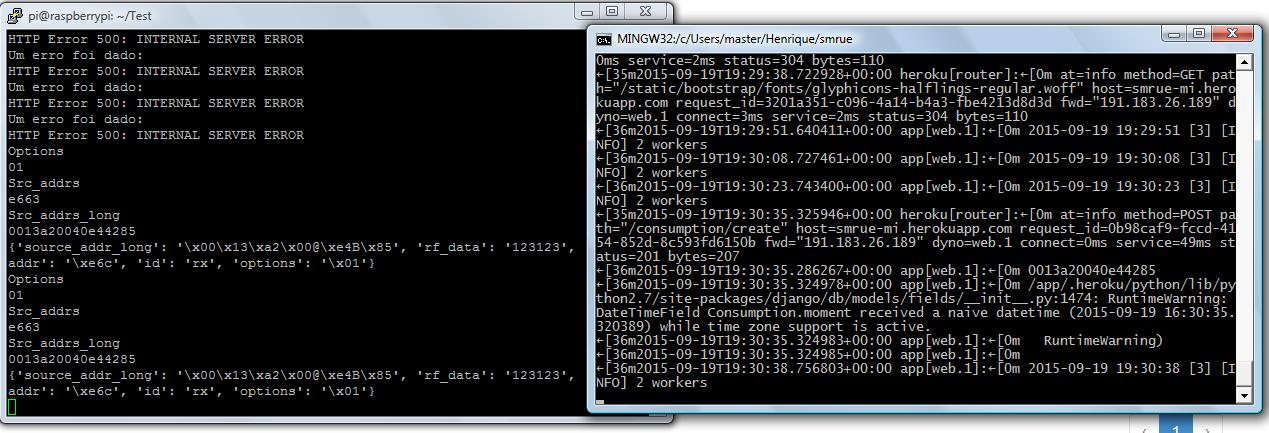
\includegraphics[width=1\textwidth]{figuras/sensor_creation.jpg}
\caption{\label{fig:sensor_creation} Teste de criação de sensor e de consumo }
\end{figure}

Em um primeiro momento, quando o sensor nem está no sistema,  o servidor retorna um erro HTTP 500 (erro de servidor), isso porque apesar do sensor ter sido criado no sistema, este não está vinculado a nenhum equipamento. Após vincular o sensor a um equipamento na tela de configurações, pode-se ver que o servidor então retorna um status 201, que mostra que o consumo foi criado.

